\section{Method}
\label{sec:method}

\pcdg controls a frozen generator through sampling-time logit projection,
category-consistent POI decoding, and terminal same-category refinement
(Figure~\ref{fig:framework}). The weights $\rho,\lambda,\beta$ enter their objectives.
\begin{figure*}[t]
  \centering
  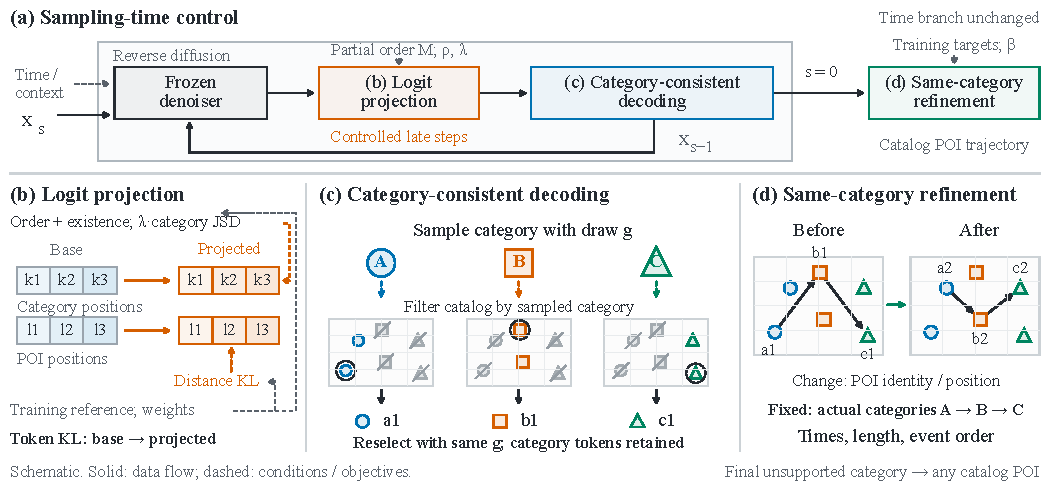
\includegraphics[width=\textwidth]{figures/framework.pdf}
  \caption{\pcdg (schematic). (a) Frozen reverse loop and terminal refinement.
  (b) Category order/existence energies and POI distance KL, anchored by base-to-projected token KL.
  (c) Category-filtered POI reselection reuses Gumbel noise.
  (d) Same-frame refinement preserves actual categories, times, length, and order.
  Dashed edges carry conditions/objectives.
  Intermediate steps allow POI masks and leave unresolved categories unfiltered.
  Unsupported final categories allow any catalog POI, permitting nonzero mismatch.}
  \Description{Four panels trace sampling-time category control. Panel a places a
  frozen denoiser, late-step logit projection, and category-consistent decoding
  inside a reverse-diffusion loop, followed by terminal same-category refinement.
  Panel b separates category and POI logit positions and their objectives.
  Panel c uses blue circles A, orange squares B, and green triangles C for three
  events. Each sampled category filters a common six-POI catalog; incompatible
  candidates are gray and crossed out. Shared-noise reselection yields a1, b1, c1.
  Panel d uses the same coordinates to replace these with a2, b2, c2 while retaining
  actual categories, times, length, and event order. A note marks the final
  unsupported-category fallback to any catalog POI.}
  \label{fig:framework}
\end{figure*}

\subsection{Backbone: conditional joint discrete diffusion}
\label{sec:method:backbone}
The current implementation uses a frozen generator whose discrete branch follows the Marionette-style diffusion point process for arrival times and conditional
discrete diffusion for categories and POIs~\cite{deng2025marionette}. Its discrete
branch represents a sequence as
$\mathbf{x}=[\textsc{start},\,k_{1:n},\,\textsc{sep},\,l_{1:n},\,\textsc{end}]$,
with a \emph{category mask} and a \emph{POI mask} identifying the two segments.
Categories and POIs use separate absorbing-state transition
matrices~\cite{austin2021d3pm}; a Transformer denoiser with an
$\mathbf{x}_0$-parameterization predicts clean-token distributions, from which
the backbone constructs the reverse-step distribution
$p(\mathbf{x}_{s-1}\!\mid\!\mathbf{x}_s)$.
We denote its per-position log-probabilities by
$\mathbf{z}\in\mathbb{R}^{V\times L}$, with vocabulary size $V$ and $L$ positions.
Projection acts on these reverse-step logits, not directly on the denoiser's
clean-token predictions. \pcdg keeps the backbone frozen and changes sampling
distributions and terminal POI assignments.

\subsection{Partial-order constraints as differentiable energies}
\label{sec:method:energy}
Given the sample-level matrix $\Mmat$, we parse it into a set of pairwise
constraints $\{(a,b): \Mmat[a,b]>\tfrac12\}$. To make a constraint differentiable
in the logits, we relax the hard categorical choice at each position into a
distribution. With temperature $T$ and (optionally) Gumbel noise $\mathbf{g}_l$,
\begin{equation}
  \boldsymbol{\pi}_l = \mathrm{softmax}\big((\mathbf{z}_l + \mathbf{g}_l)/T\big)\in\Delta^{V-1},
  \qquad l=1,\dots,L .
\end{equation}
We restrict attention to category positions $\mathcal{P}_k$ (via the category
mask) and to the category slice of the vocabulary, writing
$\pi^{\mathrm{cat}}_l(a)$ for the relaxed probability that position
$l\in\mathcal{P}_k$ takes category $a\in\mathcal{C}$. For a constraint $(a,b)$ let
$P^A_l=\pi^{\mathrm{cat}}_l(a)$ and $P^B_l=\pi^{\mathrm{cat}}_l(b)$. We define two
energies:
\begin{align}
  g^{\mathrm{ord}}_{(a,b)} &= \sum_{l\in\mathcal{P}_k}
     \Big(\textstyle\sum_{l'<l} P^B_{l'}\Big)\, P^A_l,
     \label{eq:order}\\[2pt]
  g^{\mathrm{ex}}_{(a,b)}  &= \relu\!\Big(1-\textstyle\sum_{l} P^A_l\Big)
                           + \relu\!\Big(1-\textstyle\sum_{l} P^B_l\Big).
     \label{eq:exist}
\end{align}
The \emph{order energy}~\eqref{eq:order} sums relaxed inverted-pair mass: under
independent draws at category positions it is the expected number of $b$-before-$a$
pairs. For a one-hot assignment, zero energy means no such inversion; a small
relaxed value alone does not certify the decoded sequence.
The \emph{existence energy}~\eqref{eq:exist} penalizes an
expected count below one for either constrained category, discouraging trivial
satisfaction of ordering by \emph{omitting} $a$ or $b$. Both energies are
computed only over category positions; POI logits do not enter
Eqs.~\eqref{eq:order}--\eqref{eq:exist}.

\subsection{KL-preserving augmented-Lagrangian projection}
\label{sec:method:project}
At a controlled reverse step, we project the backbone logits to reduce constraint
violations while staying close to the model's own distribution. Let
$\mathbf{y}^{(0)}=\mathbf{z}$ be the detached backbone logits and $\mathbf{y}$ a
trainable copy. The sequence-level constrained formulation is
\begin{equation}
\begin{aligned}
  \min_{\mathbf{y}}\;&\dkl\!\big(\mathrm{softmax}(\mathbf{y}^{(0)})\,\big\|\,\mathrm{softmax}(\mathbf{y})\big)\\
  \text{s.t.}\;&g^{\mathrm{ord}}_{(a,b)}\le\tau,\quad g^{\mathrm{ex}}_{(a,b)}\le\tau
  \quad\forall(a,b),
\end{aligned}
  \label{eq:constrained}
\end{equation}
where the KL term penalizes deviation from the base model; it does not guarantee
unchanged fidelity metrics. Its direction is base-to-projected: the frozen
distribution is the target argument of the implementation's KL loss.
We optimize the
augmented-Lagrangian relaxation of~\eqref{eq:constrained}: with
$\delta^{\bullet}=\relu(g^{\bullet}-\tau)$,
\begin{equation}
\begin{aligned}
  \mathcal{L}(\mathbf{y}) =\; & w_{\mathrm{kl}}\,\dkl
   + \!\!\sum_{(a,b)}\! w_{\mathrm{ord}}\Big(\lambda^{\mathrm{ord}}\delta^{\mathrm{ord}}
     + \tfrac{1}{2}\mu^{\mathrm{ord}}(\delta^{\mathrm{ord}})^2\Big)\\
   & + \!\!\sum_{(a,b)}\! w_{\mathrm{ex}}\Big(\lambda^{\mathrm{ex}}\delta^{\mathrm{ex}}
     + \tfrac{1}{2}\mu^{\mathrm{ex}}(\delta^{\mathrm{ex}})^2\Big).
\end{aligned}
\label{eq:auglag}
\end{equation}
The \emph{inner} loop uses SGD on active rows of $\mathbf{y}$ with rate $\eta$
and gradient-norm clipping. It optimizes the penalty objective without an
additional hard feasible-set projection.
An \emph{outer} loop evaluates the \emph{hard} violations
$\hat{\delta}$ (from the $\arg\max$ one-hot assignment, not the relaxation) and
updates the dual variables,
\begin{equation}
  \lambda \leftarrow \lambda + \mu\,\hat{\delta},\qquad
  \mu \leftarrow \min(\alpha\,\mu,\;\mu_{\max})\ \text{if}\ \hat{\delta}>\tau_{\mathrm{tol}},
  \label{eq:dual}
\end{equation}
using a fixed budget without early stopping in the reported runs.
The batch objective averages token KL over the full batch size but sums
order/existence penalties over active rows and relations (Appendix~\ref{app:algo}).
Hard violations determine which penalties grow. The order and existence terms
act on category positions; distance KL also updates POI logits
(\S\ref{sec:method:distance}). Hard POI-support masking belongs to the subsequent
decoder, not these order/existence energies.

\subsection{Distance-distribution regularization}
\label{sec:method:distance}
Enforcing category order perturbs the category marginals and, indirectly, the
induced spatial statistics. We therefore add a separate distance regularizer
to match the \emph{population} distribution of travel
length. From the training split only, we compute the cumulative great-circle
(Haversine) route length $d$ of every training sequence with at least two POIs and
summarize it as a soft histogram $H_{\mathrm{train}}$ over $\log(1+d)$ with fixed
Gaussian bins (the reference is content-hashed and cached, never stored in the
model). During projection, for each POI position we fix the top-$\kappa$ candidate
POIs under the backbone and draw $P$ routes with a straight-through
Gumbel-softmax (exact distance on the forward pass, a bilinear surrogate on the
backward pass), forming a differentiable route-length histogram
$H_{\mathrm{proj}}(\mathbf{y})$. We add the term
\begin{equation}
  w_{\mathrm{dist}}\,\dkl\!\big(H_{\mathrm{train}}\,\|\,H_{\mathrm{proj}}(\mathbf{y})\big)
  \label{eq:distance}
\end{equation}
to the objective~\eqref{eq:auglag}. Unlike the order/existence energies, this term
acts on \emph{POI-position} logits, and it is a batch-level distribution-matching
regularizer, not a hard constraint on each sample. It is applied only to
sequences with at least two POIs and uses an independent random stream. Its weight
is not tuned per city and is not guaranteed to improve every fidelity metric; we
quantify its effect via the \textsc{No Distance KL} ablation
(\S\ref{sec:experiments}).

\subsection{Placement in the reverse process and joint sampling}
\label{sec:method:placement}
Control runs every $f$ steps within the last $K$ reverse steps, when category
predictions inform the energies. It replaces category-position logits with
projected values and, when enabled, POI-position logits with distance-adjusted
values. Joint categorical sampling then produces the next state, optionally
using the decoder in \S\ref{sec:method:decoding}. The temporal branch is unchanged;
disabling all control stages recovers the unconstrained backbone.
Algorithm~\ref{alg:pcdg} gives the controlled step;
Appendix~\ref{app:algo} lists additional implementation settings.

\subsection{Category-consistent POI decoding}
\label{sec:method:decoding}
The category and POI segments are sampled at separate positions. A correctly
ordered category-token sequence can therefore yield POIs with different actual
categories. Since constraint metrics use $\mathrm{cat}(l)$ from the catalog,
projection of category tokens alone does not ensure activity-order control.

The decoder couples the segments within each reverse step. Let $\widetilde{\mathbf z}$
be the projected logits $\mathbf y$, or $\mathbf z$ at an uncontrolled step.
With Gumbel draw $\mathbf{g}$, first sample the full token string from these logits,
fixing category token $\hat c_l$ aligned with each POI position. Then restrict its
POI support and reselect using the \emph{same} draw:
\begin{equation}
 \hat x^{\mathrm{cc}}_l=\arg\max_{v\in S_l}(\widetilde z_{lv}+g_{lv}),
 \quad S_l=\{v:\mathrm{cat}(v)=\hat c_l\}.
 \label{eq:ccdecode}
\end{equation}
For a supported category, logits outside $S_l$ are set to $-\infty$, not a large
finite penalty. Category positions are untouched, and the sampler consumes
exactly one draw of the original shape per step. At intermediate steps the POI
mask token remains admissible; unsupported category positions are unrestricted.
At the final step, an unsupported category falls back to \emph{any catalog POI}.
Thus the implementation retains a small category--POI mismatch fraction,
$0.0034\%$--$0.0219\%$ across the six full-stack runs, rather than eliminating it.
The decoder introduces no parameters or logit prior.

\subsection{Terminal same-category geometry refinement}
\label{sec:method:geometry}
The chosen POIs determine coordinates and can shift spatial marginals
(\S\ref{sec:exp:tradeoff}). After diffusion, we therefore re-select each POI
\emph{within its own realized category}.

For every POI position we build a candidate set of at most $\kappa_g{=}32$ POIs sharing
the realized category: the originally sampled POI, the backbone's highest-scoring
candidates, the POIs closest to the generated trajectory's own centroid, and, in the
distribution-corrected variant, the most frequently visited POIs of the training
reference; duplicates are removed, the set is filled by model score, and ties are broken
by catalog id so the construction is deterministic. Stage (d) uses the original
POI, top-$15$ by score and nearest-$16$ to the centroid; stage (e) uses the original,
top-$11$, nearest-$12$, and the $8$ most visited training POIs. Scores come from one frozen,
untruncated $t{=}0$ evaluation of the backbone; reference GPS from the test split never
enters. Writing $\mathbf{w}$ for a relaxed assignment over candidates, we minimize
\begin{equation}
\begin{aligned}
  &\dkl\!\big(q\,\|\,\mathbf{w}\big)\,w_{\mathrm{fid}}
  + w_{\mathrm{d}}\,\mathrm{JSD}\big(H^{\mathrm{dist}}_{\mathrm{train}},H^{\mathrm{dist}}(\mathbf{w})\big)\\
  &\quad + w_{\mathrm{r}}\,\mathrm{JSD}\big(H^{\mathrm{rad}}_{\mathrm{train}},H^{\mathrm{rad}}(\mathbf{w})\big),
\end{aligned}
  \label{eq:geometry}
\end{equation}
where the two soft histograms are differentiable in $\mathbf{w}$ and the proposal $q$
places half of its mass on the original POI and spreads the other half over the
candidates by model score, so the fidelity term penalizes drifting away from the
backbone's preference. Optimization uses $8$ straight-through paths and a
prequalified $200$-step budget; Appendix~\ref{app:algo} gives the settings.
For the \emph{hard} output, we retain the lowest-objective assignment among the
original and $8$ optimized paths.
Empty, single-point and single-candidate positions, and batches in which the base
projection never ran, are skipped.

\paragraph{Constraint neutrality.} Because the refinement substitutes only POIs of the
same realized category, together with their catalog coordinates, and leaves category
tokens, the realized category sequence, event times, sequence lengths, event order and
all conditions unchanged \emph{per event}, every constraint-relevant statistic is
invariant by construction: OVR\textsubscript{strict}, OVR\textsubscript{skip}, pair and
category coverage, Unsat, \emph{Category}, \emph{CategoryTransition} and the
category--POI mismatch rate. We verify this numerically on every test run, requiring
agreement within $10^{-12}$. This invariance permits spatial and popularity
statistics to change, but does not guarantee a match to every reference
distribution within the candidate sets. Refinement cannot repair the category-side
divergences it preserves.

\subsection{Distribution correction}
\label{sec:method:balance}
Three scalars govern the balance between constraint strength and distributional
fidelity, all referenced to the \emph{training} reference pool only. First,
$\rho\in(0,1]$ scales the constraint term of Eq.~\eqref{eq:auglag}, so the projection
objective becomes
\begin{equation}
\begin{aligned}
  w_{\mathrm{kl}}\,\dkl
  &+ \rho\!\sum_{(a,b)}\!\mathrm{AL}\big(g^{\mathrm{ord}},g^{\mathrm{ex}};\lambda^{\bullet},\mu^{\bullet}\big)\\
  &+ w_{\mathrm{dist}}\,\dkl\big(H_{\mathrm{train}}\|H_{\mathrm{proj}}\big)
   + \lambda\,\mathcal{L}_{\mathrm{cat}} .
\end{aligned}
\label{eq:balance}
\end{equation}
Second, $\lambda\ge 0$ weights a category-side term
\begin{equation}
  \mathcal{L}_{\mathrm{cat}}=\tfrac12\big(
    \mathrm{JSD}_{\mathrm{hour}\times\mathrm{cat}}
    +\mathrm{JSD}_{\mathrm{transition}}\big),
  \label{eq:catbalance}
\end{equation}
computed from \emph{expected} counts under the relaxed assignment, without
Monte Carlo draws or additional randomness. Self-transitions are counted,
sequence boundaries excluded, and reference rows without support contribute zero.
Third, $\beta\ge 0$ adds to Eq.~\eqref{eq:geometry} a POI-side term
$\tfrac12(\mathrm{JSD}_{\mathrm{top}1000}+\mathrm{JSD}_{\mathrm{DailyLoc}})$,
where the first is an \emph{identity-aligned} top-$1000$ visitation divergence (the
generated and reference top-$1000$ sets are unioned by POI id before normalization, not
compared as sorted popularity curves) and the second a soft expected-\emph{DailyLoc}
divergence. Pre-refinement spatial samples are cached independently of $\beta$, so the
three $\beta$ settings of a batch are compared at identical upstream randomness.

The full configuration is $\rho{=}0.5$, $\lambda{=}0$, $\beta{=}1$, selected
on training-side calibration data (Appendix~\ref{app:grid}). The selected value
$\lambda=0$ describes this grid's outcome, not the absence of category-side error.

\subsection{Controlled-step algorithm}
\label{sec:method:algorithm}
Algorithm~\ref{alg:pcdg} combines the objectives above at one controlled
reverse step. Projection updates a detached copy of the reverse-step logits;
the frozen denoiser is never optimized. The inner loop uses relaxed energies,
whereas hard assignments determine the outer-loop dual updates.
After projection, category sampling and POI reselection share the same Gumbel
draw (\S\ref{sec:method:decoding}). The resulting discrete state feeds the next
reverse step. Terminal geometry refinement runs once, after diffusion ends,
and changes only same-category POI choices (\S\ref{sec:method:geometry}).

\begin{algorithm}[t]
\caption{\pcdg: one controlled reverse step}
\label{alg:pcdg}
\begin{algorithmic}[1]
\Require reverse-step logits $\mathbf z$, constraints $\Mmat$, position masks, training references
\State $\mathbf y\gets\operatorname{detach}(\mathbf z)$; initialize duals
\For{$o=1,\ldots,10$}
  \For{$j=1,\ldots,50$}
    \State Relax $\mathbf y$ with Gumbel-softmax
    \State Compute order/existence and distribution terms
    \State $\mathcal L\gets$ weighted objective in Eq.~\eqref{eq:balance}
    \State SGD on active rows of $\mathbf y$; clip gradients
  \EndFor
  \State Update duals from hard violations, Eq.~\eqref{eq:dual}
\EndFor
\State Sample category tokens; decode POIs with shared noise
\State \Return next discrete state (Eq.~\eqref{eq:ccdecode} and fallback)
\end{algorithmic}
\end{algorithm}
